\documentclass[12pt,a4paper]{scrartcl} 
\usepackage[utf8]{inputenc}
\usepackage[english,russian]{babel}
\usepackage{indentfirst}
\usepackage{misccorr}
\usepackage{graphicx}
\usepackage{amsmath}
\usepackage{url}
\usepackage{float}
\usepackage{tikz}
\usetikzlibrary{shapes.geometric, arrows.meta, positioning, calc}

\tikzset{
	block/.style={rectangle, draw, align=center, minimum width=3.6cm, minimum height=0.9cm},
	decision/.style={diamond, draw, aspect=2, align=center, inner sep=1pt},
	line/.style={-{Stealth[length=2mm]}}
}

\newlength{\ML}

\begin{document}

\begin{titlepage}
	\begin{center}
		\large
		МИНИСТЕРСТВО НАУКИ И ВЫСШЕГО ОБРАЗОВАНИЯ РОССИЙСКОЙ ФЕДЕРАЦИИ
		
		Федеральное государственное бюджетное образовательное учреждение высшего образования
		
		\textbf{АДЫГЕЙСКИЙ ГОСУДАРСТВЕННЫЙ УНИВЕРСИТЕТ}
		\vspace{0.25cm}
		
		НОК "Институт точных наук и цифровых технологий"
		
		Кафедра автоматизированных систем обработки информации и управления
		\vfill
		\vfill
		
		\textsc{Отчет по ознакомительной практике}\\[5mm]
		
		{\LARGE Численные методы. \textit{Вариант 50}}
		\bigskip
		
		1 курс, группа 1ИВТ
	\end{center}
	\vfill
	
	\settowidth{\ML}{«\underline{\hspace{0.7cm}}» \underline{\hspace{2cm}}}
	\hfill\begin{minipage}{0.5\textwidth}
		Выполнил:\\
		\underline{\hspace{\ML}} Д.\,Б.~Самогов\\
		«\underline{\hspace{0.7cm}}» \underline{\hspace{2cm}} 2026 г.
	\end{minipage}%
	\bigskip
	
	\hfill\begin{minipage}{0.5\textwidth}
		Руководитель:\\
		\underline{\hspace{\ML}} С.\,В.~Теплоухов\\
		«\underline{\hspace{0.7cm}}» \underline{\hspace{2cm}} 2026 г.
	\end{minipage}%
	\vfill
	
	\begin{center}
		Майкоп, 2026 г.
	\end{center}
\end{titlepage}

\section{Введение}

\textbf{Номер варианта: 50.}

Цель работы --- программная реализация численных методов по методическим указаниям~\cite{Zadanie-2026}: решение трансцендентного уравнения $\sqrt{1-x}=5\sin x$, системы линейных уравнений методом Гаусса и расчёт тока гальванометра по законам Кирхгофа~\cite{Uvarov-2000, Samarsky-1989, Trofimov-2015}.

Отчёт оформлен в \LaTeX{}~\cite{Lvovsky-2003}; программы написаны на языке Python~\cite{Python-2026} и содержат:
\begin{enumerate}
 \item номер варианта;
 \item исходные данные задач;
 \item ход решения с блок-схемами алгоритмов;
 \item интерпретацию результатов;
 \item выводы;
 \item программы на языке Python (фрагменты кода приведены в тексте, полные файлы --- в репозитории).
\end{enumerate}

%==============================================================================
\newpage
\section{Лабораторная работа №1. Нелинейное уравнение}

\subsection{Исходные данные}

\begin{itemize}
 \item \textbf{Вариант:} 50.
 \item \textbf{Уравнение:} $\sqrt{1-x}=5\sin x$.
 \item \textbf{Методы:} бисекция отрезка и метод секущих~\cite{Uvarov-2000}.
 \item \textbf{Точность:} $\varepsilon = 0{,}01$.
 \item \textbf{Язык программирования:} Python, файл \texttt{Program/lab1\_nonlinear.py}.
\end{itemize}

\subsection{Ход решения}

\textbf{Шаг 1.} Задаём $f(x)=\sqrt{1-x}-5\sin x$ и отделяем корни на сетке $x\le 1$: ищем интервалы $[a;b]$, где $f(a)\cdot f(b)<0$.

\textbf{Шаг 2.} На каждом интервале находим корень методом бисекции и методом секущих.

\textbf{Шаг 3.} Сравниваем результаты и проверяем $|f(x)|<\varepsilon$.

\textbf{Фрагмент программы} (файл \texttt{Program/lab1\_nonlinear.py}):
\begin{verbatim}
def f(x):
    if x > 1.0:
        return float("nan")
    return math.sqrt(1.0 - x) - 5.0 * math.sin(x)

def bisection(func, left, right, eps=0.01):
    while right - left > eps:
        middle = (left + right) / 2
        if func(left) * func(middle) <= 0:
            right = middle
        else:
            left = middle
    return (left + right) / 2

def secant(func, x0, x1, eps=0.01):
    while True:
        f0, f1 = func(x0), func(x1)
        if abs(f1) < eps:
            return x1
        x2 = x1 - f1 * (x1 - x0) / (f1 - f0)
        if abs(x2 - x1) < eps:
            return x2
        x0, x1 = x1, x2
\end{verbatim}

\subsubsection{Блок-схемы алгоритмов}

Блок-схема метода бисекции --- рис.~\ref{fig:flow-bisect}. Блок-схема общего алгоритма программы --- рис.~\ref{fig:flow-lab1}.

\begin{figure}[H]
    \centering
    \begin{tikzpicture}[
        scale=0.85, transform shape,
        block/.style={rectangle, draw, rounded corners=2pt, align=center, minimum width=2.8cm, minimum height=0.7cm},
        terminal/.style={rectangle, draw, rounded corners=10pt, align=center, minimum width=2.8cm, minimum height=0.7cm},
        decision/.style={diamond, draw, aspect=1.8, align=center, inner sep=2pt, minimum width=2.5cm},
        arr/.style={-{Stealth[length=2mm]}}
    ]
        % Центральная ветка (вход и цикл)
        \node[terminal] (start) at (0, 0) {Начало};
        \node[block] (in) at (0, -1.3) {Ввод $a$, $b$, $\varepsilon$};
        \node[decision] (dec) at (0, -3.2) {$b-a>\varepsilon$?};
        
        % Правая ветка (выход из цикла)
        \node[block] (out) at (4.5, -3.2) {$x=(a+b)/2$};
        \node[terminal] (stop) at (4.5, -4.7) {Конец};

        % Левая ветка (тело цикла)
        \node[block] (mid) at (-3.5, -4.5) {$c=(a+b)/2$};
        \node[decision] (dec2) at (-3.5, -6.2) {$f(a)f(c)\le 0$?};
        \node[block] (bset) at (-5.5, -7.8) {$b:=c$};
        \node[block] (aset) at (-1.5, -7.8) {$a:=c$};

        % Координаты для корректного обратного цикла
        \coordinate (merge) at (-3.5, -9.0);
        \coordinate (loopback) at (-3.5, -9.6); % Новая точка, чтобы увести стрелку еще ниже

        % Отрисовка стрелок
        \draw[arr] (start) -- (in);
        \draw[arr] (in) -- (dec);
        
        % Выход из цикла "нет"
        \draw[arr] (dec.east) -- node[above, scale=0.8] {нет} (out.west);
        \draw[arr] (out) -- (stop);
        
        % Вход в цикл "да"
        \draw[arr] (dec.west) -- node[above, pos=0.4, scale=0.8] {да} (mid.north);
        \draw[arr] (mid) -- (dec2);
        
        % Внутреннее ветвление f(a)f(c) <= 0
        \draw[arr] (dec2.west) -- ++(-0.5,0) node[above, scale=0.8] {да} |- (bset.north);
        \draw[arr] (dec2.east) -- ++(0.5,0) node[above, scale=0.8] {нет} |- (aset.north);
        
        % Линии вниз от присваиваний к точке слияния
        \draw[-](bset.south) -- (bset.south |- merge);
        \draw[-](aset.south) -- (aset.south |- merge);
        \draw[-](bset.south |- merge) -- (aset.south |- merge);
        
        % Линия идет от точки слияния еще ниже, затем вправо и наверх к условию цикла
        \draw[-] (merge) -- (loopback);
        \draw[arr] (loopback) -| (dec.south);

    \end{tikzpicture}
    \caption{Блок-схема метода бисекции}\label{fig:flow-bisect}
\end{figure}

\begin{figure}[H]
    \centering
    \begin{tikzpicture}[
        scale=0.8, transform shape,
        block/.style={rectangle, draw, rounded corners=2pt, align=center, minimum width=3.5cm, minimum height=0.7cm},
        terminal/.style={rectangle, draw, rounded corners=10pt, align=center, minimum width=3.5cm, minimum height=0.7cm},
        decision/.style={diamond, draw, aspect=2, align=center, inner sep=2pt, minimum width=3.0cm},
        arr/.style={-{Stealth[length=2mm]}}
    ]
        % Центральная цепочка
        \node[terminal] (start) at (0, 0) {Начало};
        \node[block] (func) at (0, -1.3) {$f(x)=\sqrt{1-x}-5\sin x$};
        \node[block] (scan) at (0, -2.6) {Сканирование $x\in[-10;1]$};
        \node[decision] (found) at (0, -4.3) {Есть\\интервалы?};

        % Блоки смещены для красивой последовательной структуры
        \node[block] (bis) at (-3.0, -5.8) {Бисекция};
        \node[block] (sec) at (-3.0, -7.2) {Секущие};
        \node[block] (empty) at (4.0, -4.3) {Сообщение};

        \node[decision] (more) at (0, -8.8) {Ещё\\интервалы?};
        \node[block] (save) at (0, -10.5) {График и скриншот};
        \node[terminal] (stop) at (0, -11.8) {Конец};

        % Координаты
        \coordinate (loopback) at (-5.5, -8.8);
        \coordinate (empty-down) at (4.0, -11.8);

        % Отрисовка
        \draw[arr] (start) -- (func);
        \draw[arr] (func) -- (scan);
        \draw[arr] (scan) -- (found);

        % Условие "Есть интервалы?"
        \draw[arr] (found.west) -| node[above, pos=0.3, scale=0.8] {да} (bis.north);
        \draw[arr] (found.east) -- node[above, scale=0.8] {нет} (empty.west);

        % Последовательный проход через оба метода
        \draw[arr] (bis.south) -- (sec.north);
        \draw[arr] (sec.south) |- (more.north);

        % Возврат цикла к первому методу (Бисекция)
        \draw[-] (more.west) -- node[above, scale=0.8] {да} (loopback);
        \draw[arr] (loopback) |- (bis.west);

        % Выход из цикла
        \draw[arr] (more) -- node[right, scale=0.8] {нет} (save);
        \draw[arr] (save) -- (stop);

        % Линия от Сообщения к Концу
        \draw[-] (empty.south) -- (empty-down);
        \draw[arr] (empty-down) -- (stop.east);

    \end{tikzpicture}
    \caption{Исправленная блок-схема программы ЛР №1}\label{fig:flow-lab1-fixed}
\end{figure}

\subsection{Результаты}

График функции и отделённые корни --- рис.~\ref{fig:lab1plot}. Найдены три корня на интервале $[-10;1]$:
\begin{itemize}
 \item $x\approx -5{,}72$;
 \item $x\approx -3{,}57$;
 \item $x\approx 0{,}18$.
\end{itemize}

\begin{figure}[H]
	\centering
	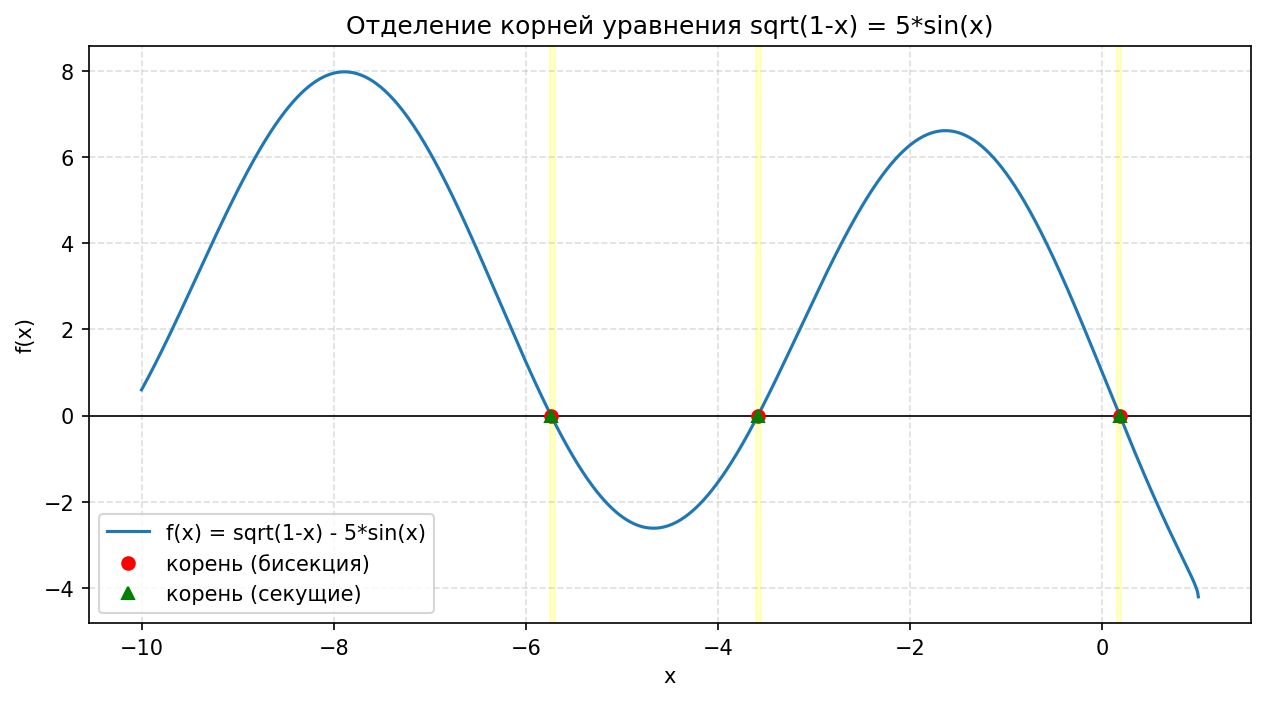
\includegraphics[width=0.95\textwidth]{lab1_plot.png}
	\caption{График $f(x)=\sqrt{1-x}-5\sin x$ и локализация корней}\label{fig:lab1plot}
\end{figure}

\begin{figure}[H]
	\centering
	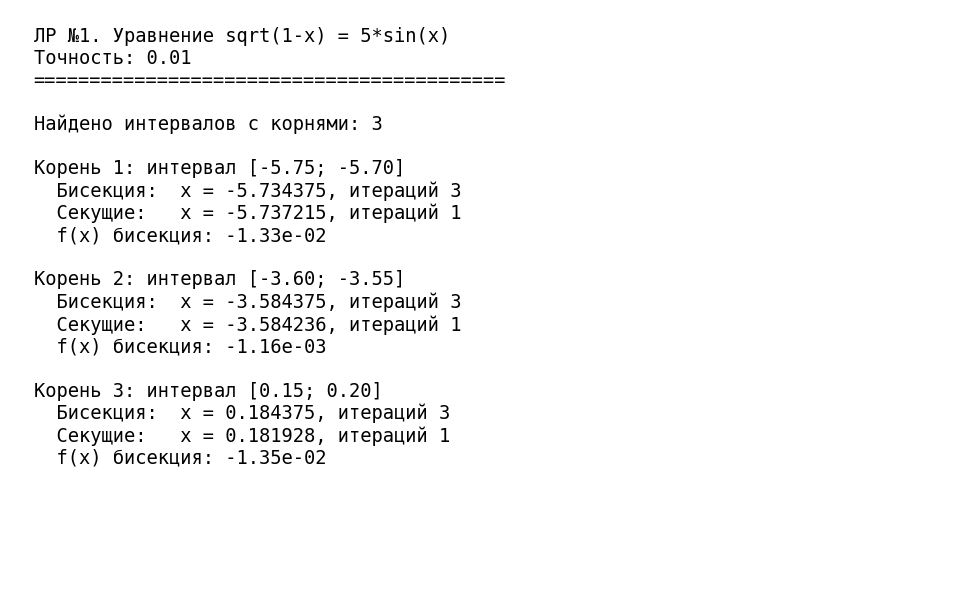
\includegraphics[width=0.75\textwidth]{lab1_output.png}
	\caption{Вывод программы ЛР №1}\label{fig:lab1out}
\end{figure}

\subsection{Интерпретация результатов}

Найденные значения $x$ --- точки пересечения графика $y=\sqrt{1-x}$ с $y=5\sin x$. При $x\le 1$ подкоренное выражение неотрицательно. Корни около $-5{,}7$, $-3{,}6$ и $0{,}2$ соответствуют трём участкам смены знака функции. Оба метода дают совпадающие результаты с точностью $0{,}01$.

\subsection{Выводы по ЛР №1}

Реализованы отделение корней, метод бисекции и метод секущих. Программа находит корни уравнения $\sqrt{1-x}=5\sin x$ с требуемой точностью; результаты подтверждены графиком и вычислением $f(x)$.

%==============================================================================
\newpage
\section{Лабораторная работа №2. Система линейных уравнений}

\subsection{Исходные данные}

\begin{itemize}
 \item \textbf{Вариант:} 50.
 \item \textbf{Метод:} Гаусса~\cite{Samarsky-1989}.
 \item \textbf{Точность:} $0{,}01$.
 \item \textbf{Матрица $A$ и вектор $\mathbf{b}$:}
\[
A=\begin{pmatrix}
0{,}78 & -0{,}02 & -0{,}12\\
0{,}02 & -0{,}86 & 0{,}04\\
0{,}12 & 0{,}44 & -0{,}72
\end{pmatrix},
\quad
\mathbf{b}=\begin{pmatrix}-0{,}56\\ 0{,}77\\ 1{,}01\end{pmatrix}.
\]
 \item \textbf{Программа:} \texttt{Program/gauss.py}.
\end{itemize}

\subsection{Ход решения}

\textbf{Шаг 1.} Формируется расширенная матрица $[A|\mathbf{b}]$.

\textbf{Шаг 2.} Прямой ход: выбор главного элемента, обнуление элементов под диагональю.

\textbf{Шаг 3.} Обратный ход: вычисление $x_n, x_{n-1}, \ldots, x_1$.

\textbf{Шаг 4.} Проверка невязок $A\mathbf{x}-\mathbf{b}$.

\textbf{Фрагмент программы} (файл \texttt{Program/gauss.py}):
\begin{verbatim}
def gauss_solve(matrix, vector):
    validate_system(matrix, vector)
    n = len(vector)
    augmented = copy_augmented(matrix, vector)

    rank = 0
    for column in range(n):
        pivot_row = find_pivot(augmented, column, rank)
        if pivot_row is None:
            continue
        # перестановка строк и обнуление столбца
        ...
        rank += 1

    solution = [0.0] * n
    for row in range(n - 1, -1, -1):
        value = augmented[row][n]
        for col in range(row + 1, n):
            value -= augmented[row][col] * solution[col]
        solution[row] = value / augmented[row][row]
    return solution
\end{verbatim}

\subsubsection{Блок-схема алгоритма}

Блок-схема метода Гаусса --- рис.~\ref{fig:flow-gauss}.

\begin{figure}[H]
    \centering
    \begin{tikzpicture}[
        scale=0.8, transform shape,
        block/.style={rectangle, draw, rounded corners=2pt, align=center, minimum width=3.5cm, minimum height=0.7cm},
        terminal/.style={rectangle, draw, rounded corners=10pt, align=center, minimum width=3.5cm, minimum height=0.7cm},
        decision/.style={diamond, draw, aspect=2, align=center, inner sep=2pt, minimum width=2.8cm},
        arr/.style={-{Stealth[length=2mm]}}
    ]
        % Центральная вертикальная ось
        \node[terminal] (start) at (0, 0) {Начало};
        \node[block] (in) at (0, -1.3) {Ввод $A$, $\mathbf{b}$};
        \node[block] (val) at (0, -2.6) {Проверка размерности};
        \node[block] (aug) at (0, -3.9) {Матрица $[A|\mathbf{b}]$};
        \node[block] (col) at (0, -5.2) {$k:=1$};
        \node[decision] (more) at (0, -6.9) {$k\le n$?};

        % Левая ветка (Тело цикла - Прямой ход Гаусса)
        \node[block] (pivot) at (-4.5, -6.9) {Главный элемент};
        \node[block] (zero) at (-4.5, -8.3) {Обнуление столбца $k$};
        \node[block] (inc) at (-4.5, -9.7) {$k:=k+1$};

        % Правая ветка (Выход из цикла - Обратный ход)
        \node[block] (back) at (4.5, -6.9) {Обратный ход};
        \node[block] (res) at (4.5, -8.3) {Невязки $A\mathbf{x}-\mathbf{b}$};
        \node[block] (out) at (4.5, -9.7) {Вывод $\mathbf{x}$};
        \node[terminal] (stop) at (4.5, -11.0) {Конец};

        % Точка для красивого изгиба стрелки возврата под циклом
        \coordinate (loopback) at (-4.5, -10.8);

        % Отрисовка стрелок центральной оси
        \draw[arr] (start) -- (in);
        \draw[arr] (in) -- (val);
        \draw[arr] (val) -- (aug);
        \draw[arr] (aug) -- (col);
        \draw[arr] (col) -- (more);

        % Ветвление цикла
        \draw[arr] (more.west) -- node[above, scale=0.8] {да} (pivot.east);
        \draw[arr] (more.east) -- node[above, scale=0.8] {нет} (back.west);

        % Движение по левой ветке (вниз)
        \draw[arr] (pivot) -- (zero);
        \draw[arr] (zero) -- (inc);

        % КОРРЕКТНЫЙ ВОЗВРАТ ЦИКЛА: вниз, вправо и строго вверх в ромб
        \draw[-] (inc.south) -- (loopback);
        \draw[arr] (loopback) -| (more.south);

        % Движение по правой ветке (вниз к концу)
        \draw[arr] (back) -- (res);
        \draw[arr] (res) -- (out);
        \draw[arr] (out) -- (stop);

    \end{tikzpicture}
    \caption{Блок-схема метода Гаусса}\label{fig:flow-gauss}
\end{figure}

\subsection{Результаты}

\[
x_1\approx -1{,}08,\quad x_2\approx -1{,}02,\quad x_3\approx -2{,}21.
\]

Невязки $\approx 10^{-16}$. График и вывод программы --- рис.~\ref{fig:gaussplot}, \ref{fig:gaussout}.

\begin{figure}[H]
	\centering
	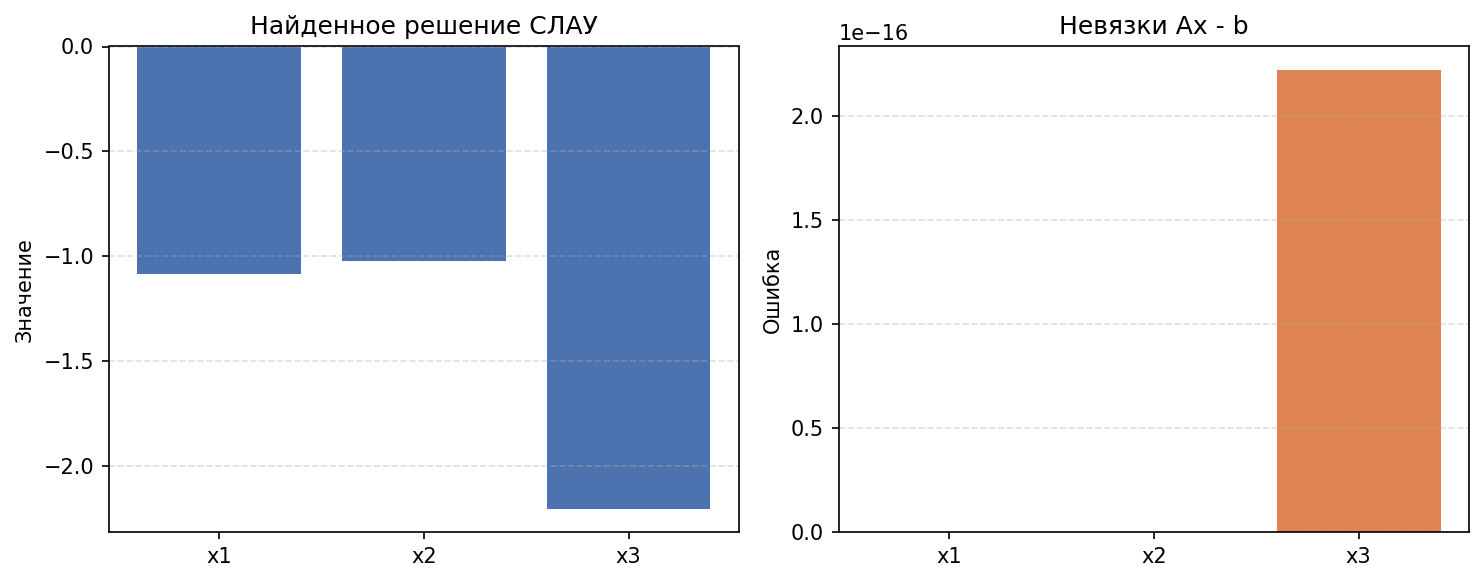
\includegraphics[width=0.9\textwidth]{gauss_solution.png}
	\caption{Решение СЛАУ варианта 50}\label{fig:gaussplot}
\end{figure}

\begin{figure}[H]
	\centering
	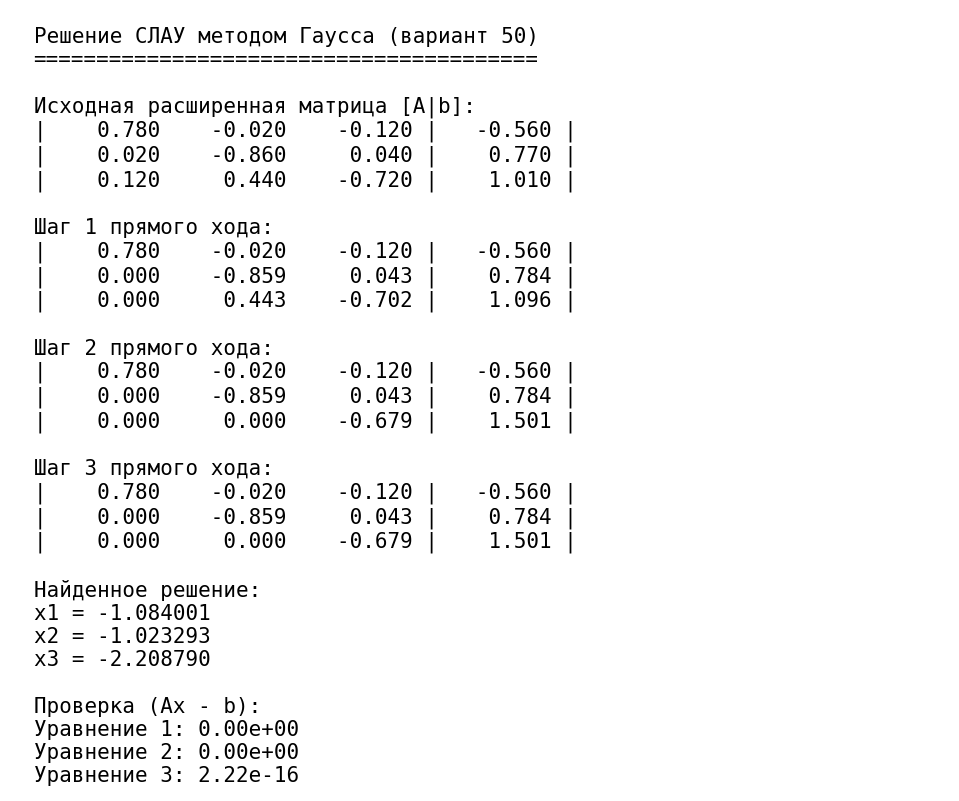
\includegraphics[width=0.85\textwidth]{gauss_output.png}
	\caption{Вывод программы метода Гаусса}\label{fig:gaussout}
\end{figure}

\subsection{Интерпретация результатов}

Вектор $\mathbf{x}$ --- набор неизвестных системы трёх линейных уравнений. Все три компоненты отрицательны: $x_1\approx -1{,}08$, $x_2\approx -1{,}02$, $x_3\approx -2{,}21$. Малые невязки подтверждают, что найденный вектор удовлетворяет исходной системе $A\mathbf{x}=\mathbf{b}$.

\subsection{Выводы по ЛР №2 (задание 1)}

Метод Гаусса реализован с проверкой входных данных и выбором главного элемента. Система варианта~50 имеет единственное решение, найденное с высокой точностью.

%==============================================================================
\newpage
\section{Лабораторная работа №2. Задание 2.5}

\subsection{Исходные данные}

\begin{itemize}
 \item \textbf{Задача:} 2.5.
 \item $\xi_1=2$~В, $\xi_2=1$~В.
 \item $R_1=1$~кОм, $R_2=500$~Ом, $R_3=200$~Ом, $R_g=200$~Ом.
 \item Внутренними сопротивлениями источников пренебрегаем.
 \item \textbf{Программа:} \texttt{Program/lab2\_galvanometer.py}.
\end{itemize}

\subsection{Ход решения}

Цепь содержит три параллельные ветви: левая ($R_2$, $\xi_1$, $R_3$), средняя ($R_1$) и правая ($R_g$, $\xi_2$)~\cite{Trofimov-2015}. По законам Кирхгофа:
\[
I_{R_1}(R_2+R_3+R_g+R_1)=E_1 R_g + E_2(R_2+R_3),
\]
\[
I_g = -I_{R_1} - I_{\text{лев}}.
\]
Подстановка даёт $I_g\approx 0{,}288$~мА.

\textbf{Фрагмент программы} (файл \texttt{Program/lab2\_galvanometer.py}):
\begin{verbatim}
E1, E2 = 2.0, 1.0
R1, R2, R3, RG = 1000.0, 500.0, 200.0, 200.0

def solve_galvanometer_25():
    denom = R1*(R2+R3) + R1*RG + (R2+R3)*RG
    i_r1 = (E1*RG + E2*(R2+R3)) / denom
    i_left = (i_r1*R1 - E1) / (R2+R3)
    i_g = -i_left - i_r1
    return {"I_galvanometer_mA": i_g * 1000.0}
\end{verbatim}

\subsubsection{Блок-схема алгоритма}

Блок-схема программы --- рис.~\ref{fig:flow-circuit}.

\begin{figure}[H]
	\centering
	\begin{tikzpicture}[
	    node distance=0.9cm and 1.4cm,
	    scale=0.82, transform shape,
	    block/.style={rectangle, draw, rounded corners=2pt, align=center, minimum width=3.0cm, minimum height=0.8cm}
	]
		\node (start) [block] {Начало};
		\node (data) [block, right=of start] {$E_1,E_2$,\\$R_1,R_2,R_3,R_g$};
		\node (den) [block, right=of data] {Знаменатель\\цепи};
		\node (ir1) [block, right=of den] {$I_{R_1}$};
		\node (ileft) [block, below=of ir1] {$I_{\text{лев}}$};
		\node (ig) [block, left=of ileft] {$I_g=-I_{R_1}-I_{\text{лев}}$};
		\node (print) [block, left=of ig] {Вывод, мА};
		\node (shot) [block, left=of print] {Скриншот};
		\node (stop) [block, left=of shot] {Конец};

		\draw[line] (start) -- (data);
		\draw[line] (data) -- (den);
		\draw[line] (den) -- (ir1);
		\draw[line] (ir1) -- (ileft);
		\draw[line] (ileft) -- (ig);
		\draw[line] (ig) -- (print);
		\draw[line] (print) -- (shot);
		\draw[line] (shot) -- (stop);
	\end{tikzpicture}
	\caption{Блок-схема программы задачи 2.5}\label{fig:flow-circuit}
\end{figure}

\subsection{Результаты}

Ток гальванометра: $I_g\approx 0{,}288$~мА. Скриншот --- рис.~\ref{fig:circuit}.

\begin{figure}[H]
	\centering
	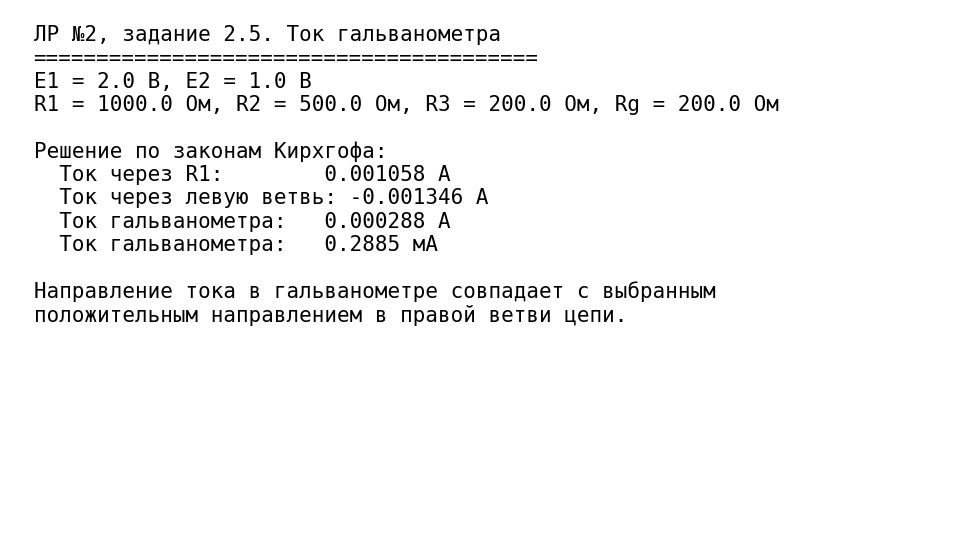
\includegraphics[width=0.85\textwidth]{lab2_galvanometer_output.png}
	\caption{Вывод программы задачи 2.5}\label{fig:circuit}
\end{figure}

\subsection{Интерпретация результатов}

Ток $0{,}288$~мА --- небольшой ток, протекающий через гальванометр из-за разности потенциалов между параллельными ветвями цепи. При других значениях сопротивлений ток мог бы обнулиться (условие баланса моста).

\subsection{Выводы по заданию 2.5}

Задача 2.5 решена аналитически и проверена программой. Ток через гальванометр составляет $0{,}288$~мА.

%==============================================================================
\newpage
\section{Общие выводы}

\begin{enumerate}
 \item Выполнены все задания \textbf{варианта 50}: нелинейное уравнение, СЛАУ методом Гаусса, расчёт тока гальванометра (задача 2.5).
 \item Составлены программы на Python с контролем входных данных (файлы \texttt{lab1\_nonlinear.py}, \texttt{gauss.py}, \texttt{lab2\_galvanometer.py}).
 \item Построены блок-схемы алгоритмов (рис.~\ref{fig:flow-bisect}--\ref{fig:flow-circuit}).
 \item Результаты интерпретированы в терминах исходных задач и подтверждены графиками и проверками.
\end{enumerate}

\newpage
\section{Список литературы}

\begin{thebibliography}{9}
\bibitem{Zadanie-2026}Методические указания по ознакомительной практике «Численные методы». Вариант~50. Файл \texttt{zadanie.pdf}.
\bibitem{Uvarov-2000}Уваров, С. Математические методы физики / С.\,К.~Уваров, Е.\,Б.~Барулин, И.\,Л.~Розенталь. --- М.: Атомиздат, 2000. --- Гл.~о методах решения нелинейных уравнений (бисекция, секущие).
\bibitem{Samarsky-1989}Самарский, А. Численные методы / А.\,А.~Самарский, А.\,В.~Гулин. --- 2-е изд. --- М.: Наука, 1989. --- Гл.~о методе Гаусса для СЛАУ.
\bibitem{Trofimov-2015}Трофимова, Т. Курс общей физики. Электричество и магнетизм / Т.\,И.~Трофимова. --- М.: Академия, 2015. --- Законы Кирхгофа, расчёт цепей постоянного тока.
\bibitem{Kalashnikov-2004}Калашников, С. Общая физика. Т.~2. Электричество и магнетизм / С.\,Г.~Калашников. --- М.: Физматлит, 2004. --- Задачи на ток в ветвях цепи и гальванометр.
\bibitem{Python-2026}Документация Python~3 [Электронный ресурс]. URL: \url{https://docs.python.org/3/} (дата обращения: 21.06.2026).
\bibitem{Matplotlib-2026}Matplotlib: Visualization with Python [Электронный ресурс]. URL: \url{https://matplotlib.org/} (дата обращения: 21.06.2026).
\bibitem{Lvovsky-2003}Львовский, С. Набор и верстка в системе \LaTeX{} / С.\,М.~Львовский. --- 3-е изд. --- М.: Академический проект, 2003.
\end{thebibliography}

\end{document}